% Section content template for individual Educative lessons
% This file contains the actual content for a specific section
% Generated from Educative API section content

% Section: Getting Ready: The Restaurant Management System
% Section ID: 4775481582026752
% Section Slug: getting-ready-the-restaurant-management-system
% Generated: 2025-12-14T12:22:34.346735

A \textbf{restaurant management system} is a software platform used to manage various aspects of a restaurant's operations, such as food and beverage sales, table reservations, billing, and seating arrangements. It supports various restaurant types---from quick-service outlets to fine dining---and helps streamline service and improve customer satisfaction.
\\
The system allows managers to monitor available tables, handle reservations, and generate bills---all from a central interface.

\begin{figure}[htbp]
 \centering
 \begin{subfigure}[b]{0.48\textwidth}
 \centering
 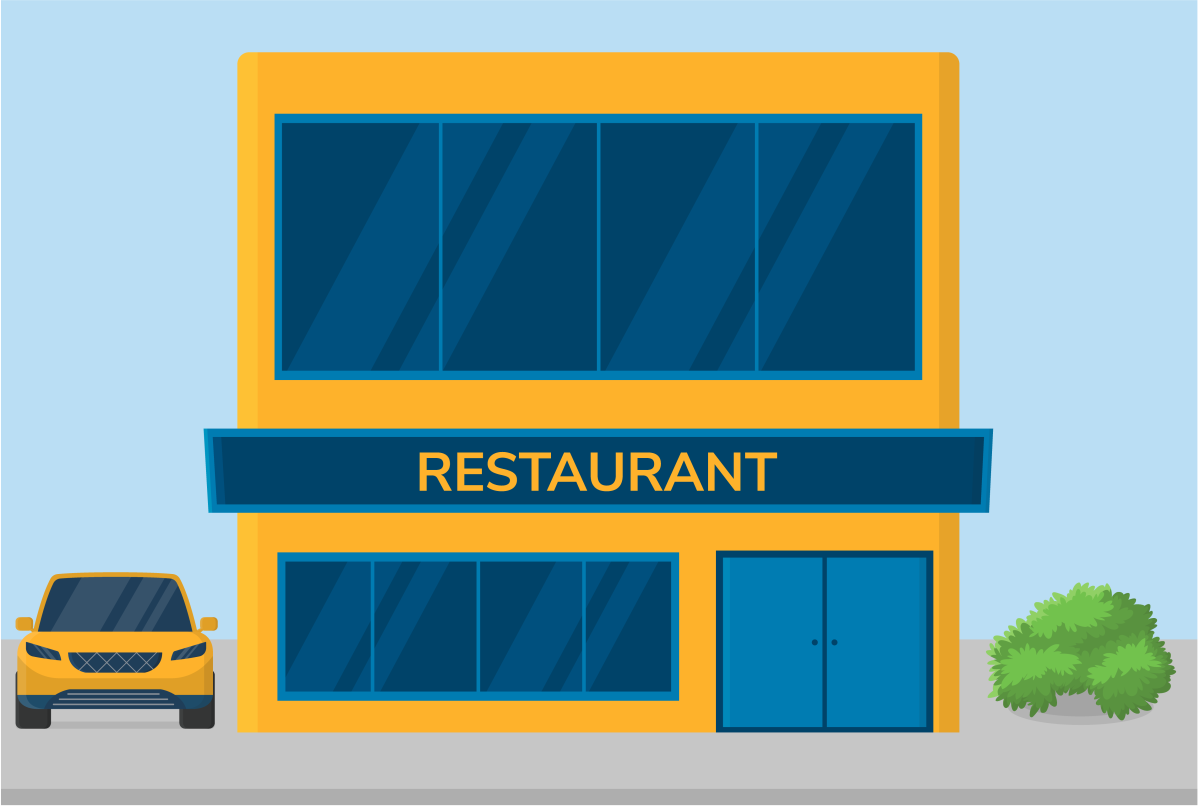
\includegraphics[width=\textwidth]{Images/chapter_21/section_4775481582026752/5939364661297152.png}
 \caption{An outer view of the restaurant}
 \end{subfigure}
 \hfill
 \begin{subfigure}[b]{0.48\textwidth}
 \centering
 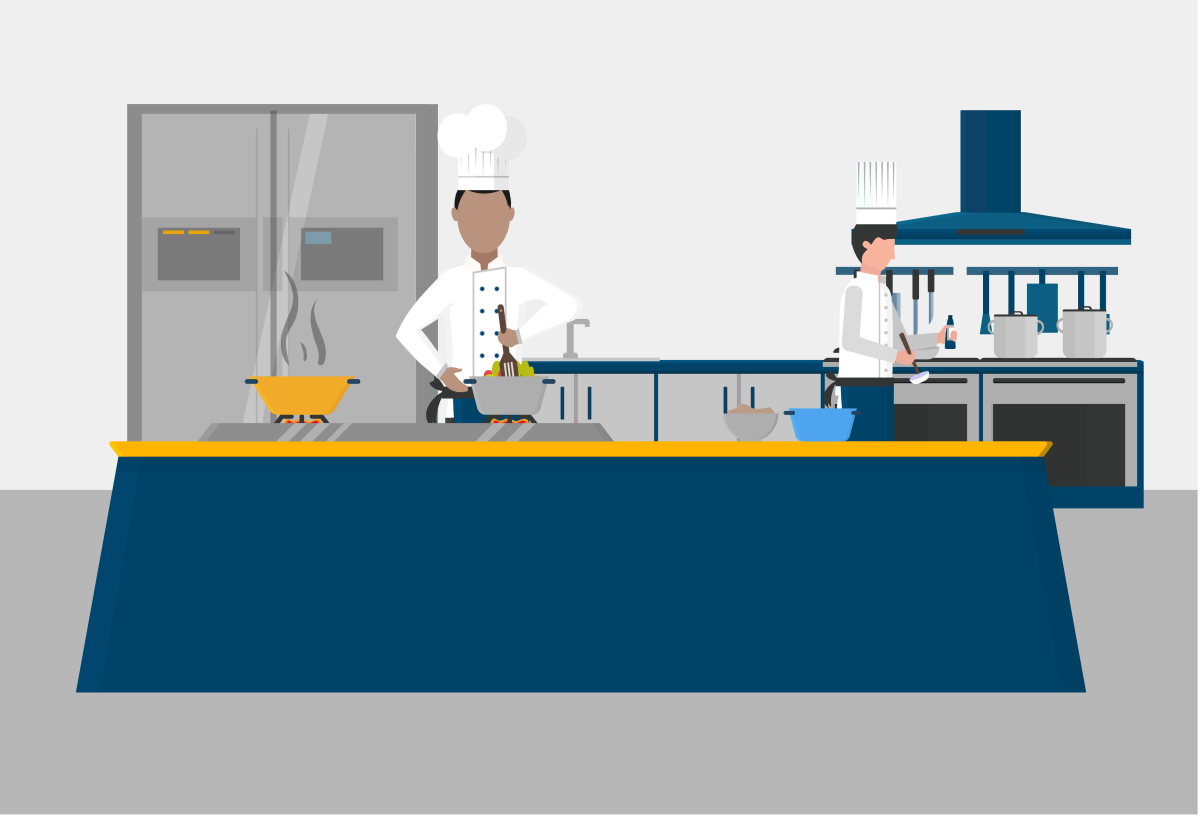
\includegraphics[width=\textwidth]{Images/chapter_21/section_4775481582026752/5432386453241856.png}
 \caption{The food being prepared for the customers}
 \end{subfigure}
\end{figure}

\begin{figure}[htbp]
 \centering
 \begin{subfigure}[b]{0.48\textwidth}
 \centering
 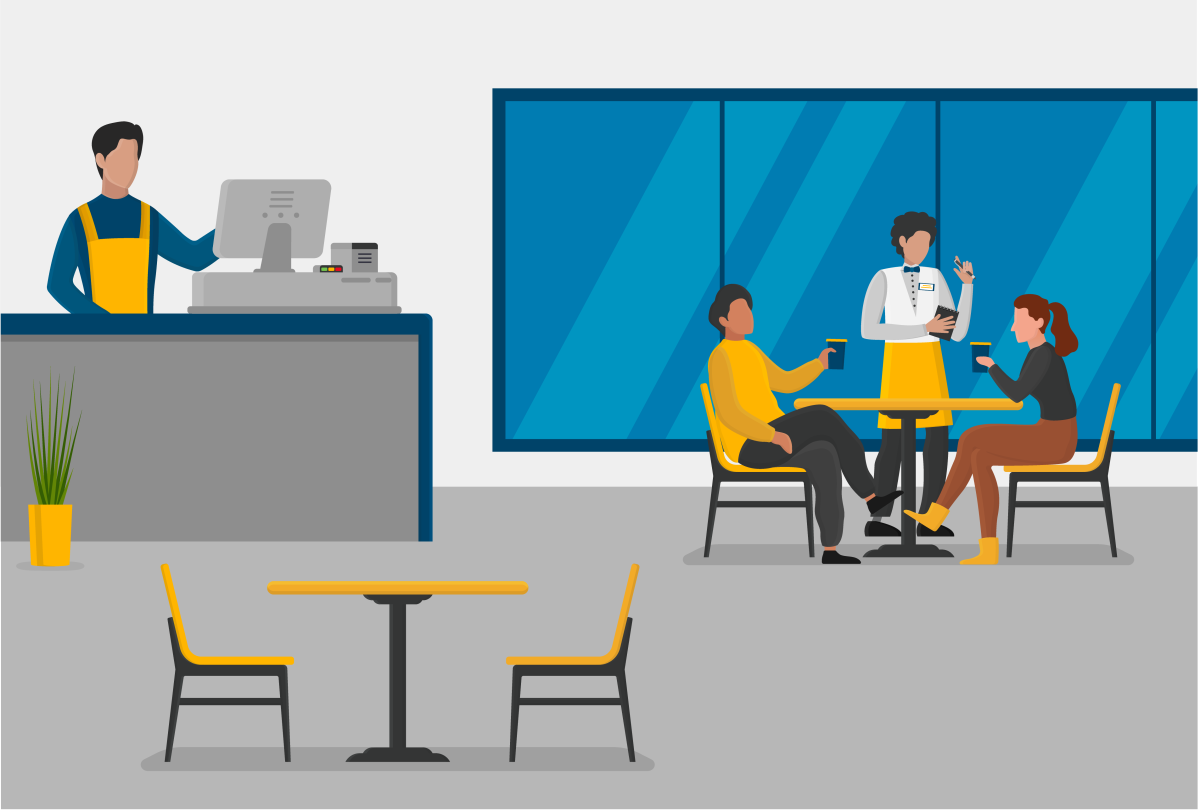
\includegraphics[width=\textwidth]{Images/chapter_21/section_4775481582026752/5603472616718336.png}
 \caption{A service being provided to the customers}
 \end{subfigure}
\end{figure}

\subsection{Expectations from the interviewee}\label{RVh3bgq_XFsdaf_qB2j1n}
\\
A restaurant management system has several components, each with specific constraints and requirements. The following provides an overview of some of the main expectations that the interviewer will want to hear you discuss in more detail during the interview.

\subsubsection{Restaurant services}\label{gziQE3vBlg5PeWmHt5RsU}
\\
To better understand the services offered by a restaurant management system, you may ask the interviewer the following questions:

\begin{enumerate}
\item
\protect\phantomsection\label{JglEp1o3bPfp8o1B3dCXi}
Does the restaurant provide a delivery service?
\item
\protect\phantomsection\label{44zo0ov2hk5PoWK-d1gEC}
Can a customer place an online order?
\item
\protect\phantomsection\label{0eyb2KHawyg3zEfGZL6B4}
Does the restaurant accept online/card payments?
\end{enumerate}

\subsubsection{Restaurant management}\label{w85vLBFYtNqodud0mUXJw}
\\
Ask these to clarify structural and operational needs:

\begin{itemize}
\item
\protect\phantomsection\label{0VxeFN4q0AUhFxkIjKBhc}
Can the restaurant have multiple branches?
\item
\protect\phantomsection\label{rUD4O-2Q6YYa_gh9k0mfM}
Do we need to account for inventory management?
\end{itemize}

\subsection{Design approach}\label{MpNP2-BX-3jSqtP87UF3x}
\\
We'll design this restaurant management system using the bottom-up approach. Therefore, we'll follow the steps below:

\begin{itemize}
\item
\protect\phantomsection\label{UIdRwl-OZrAD7XgRBltFf}
Identify and design the smallest components---the table, table seat, meal, meal item, and seating chart.
\item
\protect\phantomsection\label{vcdYBTKLnBUQetpogfmLq}
Use these small components to design bigger components---the menu, branch, and restaurant.
\item
\protect\phantomsection\label{85L-86xuuinkjVeeoXN0l}
Repeat the steps above until we design the whole restaurant management system.
\end{itemize}

\subsection{Design pattern~}\label{LldEllo7t25aIKUG6troB}
\\
During an interview, discussing the design patterns under which the restaurant management system falls is always a good practice. Stating the design patterns gives the interviewer a positive impression and shows that the interviewee is well-versed in the advanced concepts of object-oriented design.
\\
Try to answer the following question. If you are not familiar with design patterns, don't worry! You can learn about them by asking, ``Define design patterns.''

\textbf{Question:}

Which design pattern(s) should be used to design a restaurant management system? Please elaborate on your choice(s).

Let's explore the requirements of the restaurant management system in the next lesson.

% End of section content